\documentclass[border=6pt]{standalone}
\usepackage[T1]{fontenc}
\usepackage[utf8]{inputenc}
\usepackage{mathptmx}
\usepackage{amsmath,amssymb,amsfonts,mathrsfs}
\usepackage[dvipsnames]{xcolor}
\usepackage{tikz}
\usetikzlibrary{calc,positioning,arrows.meta,decorations.pathreplacing,
                decorations.markings,matrix,fit,backgrounds,shapes.misc}
\renewcommand{\sl}{\mathfrak{sl}}
\newcommand{\Uq}{U_q(\sl_2)}
\newcommand{\qint}[1]{[#1]_q}
\newcommand{\Rcheck}{\check{R}}
\definecolor{accent}{RGB}{59,91,146}
\definecolor{accentsoft}{RGB}{155,180,216}
\definecolor{oddsign}{RGB}{138,40,132}
\tikzset{
  strand/.style={line width=1pt, accent!80!black},
  rbox/.style={draw=accent!70!black, fill=accentsoft!55, rounded corners=2pt,
               line width=0.8pt, minimum height=6mm},
  rdot/.style={circle, fill=accent, inner sep=1.6pt},
  knode/.style={circle, draw=accent!70!black, fill=accentsoft!45,
                line width=0.8pt, minimum size=7mm, font=\small},
  kedge/.style={accent!70!black, line width=0.9pt},
  faredge/.style={oddsign!75!black, line width=0.9pt, densely dashed},
  glabel/.style={font=\footnotesize, accent!60!black},
}
\begin{document}
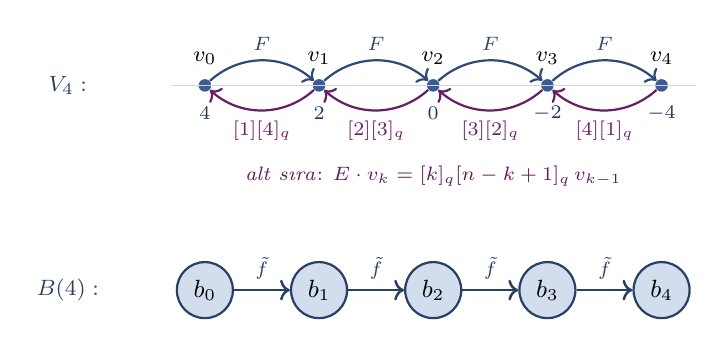
\begin{tikzpicture}[x=1.45cm,y=1cm]
  % --- Agirlik diyagrami V_4 ---
  \node[glabel, accent!70!black] at (-1.2,0) {$V_4:$};
  \foreach \k/\w in {0/4,1/2,2/0,3/-2,4/-4}{
    \node[rdot] (v\k) at (\k,0) {};
    \node[font=\footnotesize] at (\k,0.34) {$v_{\k}$};
    \node[font=\scriptsize, accent!60!black] at (\k,-0.36) {$\w$};
  }
  \draw[accent!25!white, line width=0.6pt] (-0.3,0) -- (4.3,0);
  % F oklari (ustte)
  \foreach \a/\b in {0/1,1/2,2/3,3/4}{
    \draw[->, accent!80!black, line width=0.8pt]
      (v\a) to[bend left=42] node[above, font=\scriptsize] {$F$} (v\b);
  }
  % E oklari (altta), katsayilar [k][n-k+1]
  \foreach \a/\b/\c in {1/0/{[1][4]},2/1/{[2][3]},3/2/{[3][2]},4/3/{[4][1]}}{
    \draw[->, oddsign!75!black, line width=0.8pt]
      (v\a) to[bend left=42] node[below, font=\scriptsize] {$\c_q$} (v\b);
  }
  \node[font=\scriptsize, oddsign!70!black] at (2,-1.15)
    {\emph{alt sıra}: $E\cdot v_k=\qint{k}\qint{n-k+1}\,v_{k-1}$};

  % --- Kristal B(4) ---
  \begin{scope}[yshift=-2.6cm]
    \node[glabel, accent!70!black] at (-1.2,0) {$B(4):$};
    \foreach \k in {0,1,2,3,4}{
      \node[knode] (b\k) at (\k,0) {$b_{\k}$};
    }
    \foreach \a/\b in {0/1,1/2,2/3,3/4}{
      \draw[->, kedge] (b\a) -- node[above, font=\scriptsize] {$\tilde f$} (b\b);
    }
  \end{scope}
\end{tikzpicture}
\end{document}
